\section{Power output stage}
As the power control of the coil is digital, a power transistor has been used to turn it on and off from the microcontroller. The coil is attached between the filtered 12V rail and the transistor's collector, while the transistor's base is attached to the output pin of the microcontroller in a common-emitter configuration. A LM395T transistor has been chosen, which includes a built-in 500$\Omega$ resistor in series with the base pin and a reverse-biased protection diode between emitter and collector. The high $\beta$ of the transistor makes it possible to control the coil's current using the 3.3V GPIO output of the microcontroller with a current of only 5mA. The dropout voltage on the transistor when turned on has been measured to be about 1.5V, which means about 0.5W of dissipation at full-on, which is fully sustainable with no external disspator on its TO-220 package.

A reverse-biased diode has also been added between the transistor's collector and the 12V rail: this is to protect the circuit from inductive voltage spikes and let the coil discharge easily when it's turned off. This must be considered when taking into account the control system, as it implies that charging and discharging rates will be very different each other.

Keeping in mind the previously stated model for this output stage, it can be seen that the coil acts as an integrator and sees as an input the pulses from the microcontroller. The circuit thus acts as a Delta-Sigma DAC: the microcontroller modulates a stream of pulses of fixed width of $10^{-4} s$, each pulse being 0 or 1 depending on whether the desired reference (analog) signal to apply to the coil is, at each time instant, higher or lower than the integrator's (i.e. the coil's) actual output value. The feedback for this DAC, i.e. the output of the coil, is not measured but simulated from the microcontroller.


\begin{figure}[htbp]
\centering
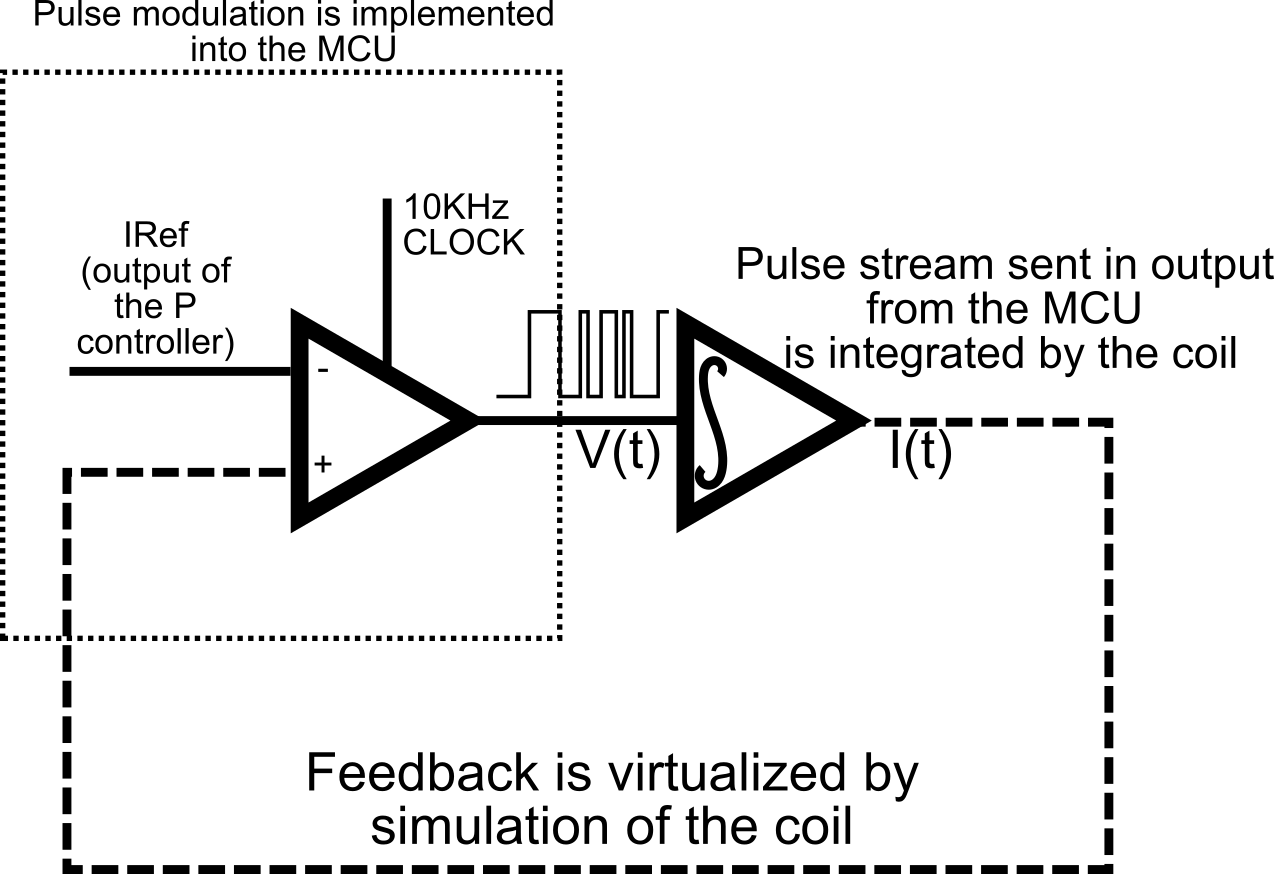
\includegraphics[width=4in]{Graphics/DSModulator.png}
\caption{Schema of the analog control part: the MCU is used to implement a form of Delta-Sigma pulse modulation in order to control the current on the coil.}
\end{figure}

\begin{figure}[htbp]
\centering
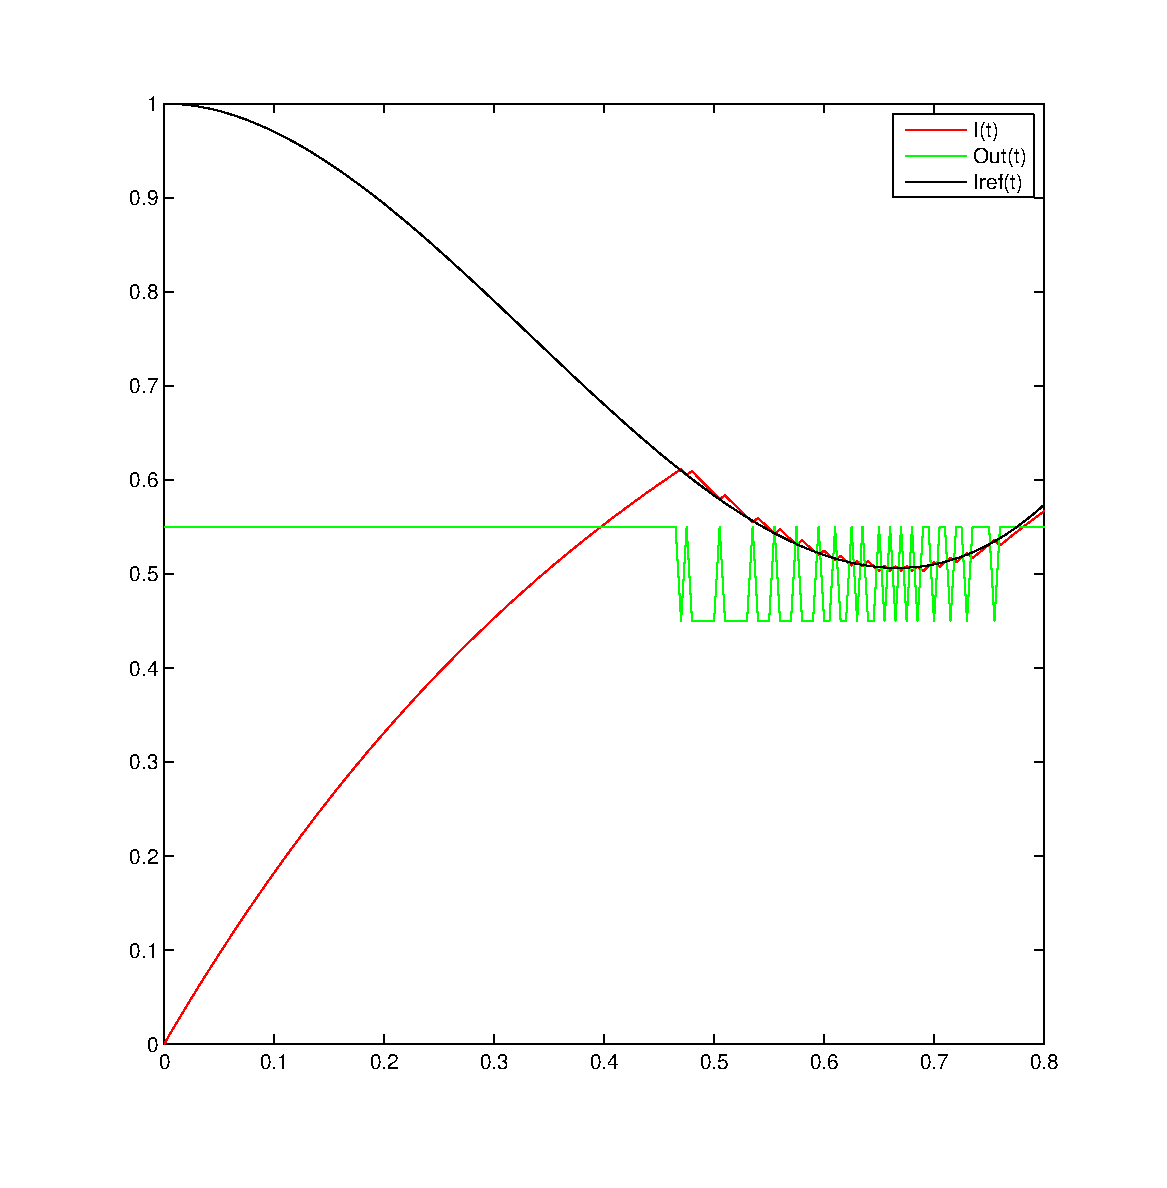
\includegraphics[width=4in]{Graphics/SD}
\caption{Simulation of the pulse modulation showing that the MCU will reach a stable output current by tracking the reference current and modulating the density of binary pulses.}
\end{figure}


